\chapter{About CodeBall 2018 world}

\newcommand{\const}[1]{\texttt{#1}}

\section{General concept of the game and the rules of the tournament}

This competition gives you an opportunity to test your programming skills,
by creating an artificial intelligence (strategy)
controlling a team of robots in a special world
(you can learn about details of the CodeBall 2018 world in later sections).
In different stages of the contest your team will consist of 2 or 3 robots,
and using nitro may or may not be available.
All robots have same parameters and are spheres, initial location is guaranteed to be symmetrical.
There is also a ball in the game.

In each game you are to compete against another player's strategy.
You team's goal --- is to score the ball into opponent's net and defend your own.
Team who has scored most goals is the winner.
Game can also be tied if both teams scored same number of goals.

The championship is held in several stages

The tournament is held in several stages preceded by a qualification in the Sandbox.
Sandbox is a competition that takes place throughout the championship.
The player has a certain rating value -- an indicator of how successful
his strategy is involved in games within each stage.

The initial value of the rating in the Sandbox is $1200$. At the end of the game this value can both be increased and decreased. At the same time victory
over a weak (with a low rating) opponent gives a small increase, also the defeat from a strong opponent slightly decreases your
rating. Over time the rating in the Sandbox becomes more and more inert, which makes it possible to decrease the impact of random long series of victories or
defeats on the participant's place, but at the same time makes it difficult to change his position with a significant improvement in strategy. To cancel such effect
the participant can reset the variability of the rating to the initial state when sending a new strategy, including the corresponding
option. If the new strategy is adopted, the rating system of the participant will fall dramatically after the next game in the Sandbox, however,
further participation in games will quickly recover and even become higher if your strategy has really become more effective. It is not recommended
to use this option with minor, incremental improvements to your strategy, as well as in cases where a new strategy
insufficiently tested and the effect of changes in it is not known reliably.

The initial value of the rating at each main stage of the tournament is $0$. For each game the participant receives a certain number of rating points
depending on the occupied place (a system similar to that used in the championship ``Formula-1’’). If two or more participants share
some place, then the total number of rating points for this place and for the following $\texttt{number\_of\_such\_members}-1$ of places is shared
equally among these participants. For example, if two participants share the first place, then each of them will receive half of the rating points number
for the first and second places. When sharing rounding always takes place in a smaller direction. More detailed information about the stages of the tournament will be
provided in the announcements on the project website.

First all participants can participate only in the games that take place in the Sandbox. Players can send their strategies to the Sandbox, and
the last one taken from them is taken by the system for participation in qualifying games. Each player participates in approximately one qualifying
game for an hour. The jury reserves the right to change this interval based on the throughput of the testing system, but for
the majority of participants it remains constant. There are a number of criteria by which the interval of participation in qualifying games
can be increased for a specific player. For every N-th full week that has elapsed since the player sent the last strategy, the interval
of participation for this player is increased by N basic test intervals. Only the strategies adopted by the system are taken into account. An additional penalty which is equal to $20\%$ from the basic testing interval is charged in the Sandbox for each strategy ``crash’’ in $10$ last games.
More details about the causes of the strategy ``crashing’’ can be found in the following sections. The player’s participation interval in the Sandbox can not become bigger than a day.

Games in the Sandbox are held according to a set of rules corresponding to the rules of an accidental past stage of the tournament or to the rules of the next
(current) stage. At the same time, the closer the rating value of the two players rating within the Sandbox, the more likely that they will be in the
one game. The Sandbox starts before the start of the first stage of the tournament and ends after some time after the final stage (see the schedule
of stages to clarify the details). In addition, the Sandbox is frozen during the stages of the tournament. Following the results of the games in the Sandbox
there is a selection for participation in Round 1, which will involve $1080$ of participants with the highest rating at the beginning of this stage of the tournament
(if the rating is equal, priority is given to the player who previously sent the latest version of his strategy), as well as an additional selection to
the next stages of the tournament, including the Finals.

Tournament stages:
\begin{itemize}
      \item
            In \textbf{Round 1} you will learn the rules of the game and master the control of the robots.
            You are given $2$ robots, same as your opponent.
            The task is --- score goals! It's simple.
            Round 1, as all further stages, consists of two parts, between which there will be a short break (with the renewal of the Sandbox work), which
            allows to improve its strategy. The last strategy sent by the player before the beginning of this part is selected for the games in each part.
            Games are conducted in waves. In each wave, each player participates exactly in one game. The number of waves in each part is determined by
            the capabilities of the testing system, but it is guaranteed that it will not be less than ten. $300$ highest rated participants
            will be held in Round 2. Also in Round 2 there will be an additional selection of $60$ participants with the highest rating in the Sandbox (at the moment
            of Round 2 beginning) among those who did not passed according to the results of Round 1.
      \item
            In \textbf{Round 2} you have to improve your robot's skills.
            Now they can use nitro.
            Also, nitro packs spawn on the map that refill robot's nitro.
            The task is further complicated
            that after summarizing the Round 1, the part of the weak strategies will be eliminated and you will have to confront stronger opponents. According
            to the results of Round 2 of the best $50$ strategies will reach the Finals. Also in the Finals there will be an additional selection of $10$ participants with
            the highest rating in the Sandbox (at the beginning of the Finals) from those who did not go through the main tournament.
      \item
            \textbf{Finals} is the most important stage. After the selection, held following the results of the first two stages, the strongest participants will be remained.
            Also, not each team has $3$ robots.
            The system of holding the Finals has its own peculiarities. The stage is still
            divided into two parts, but they will no longer consist of waves. In each part of the stage, games will be played between all pairs
            of Finals participants. If the time and capabilities of the testing system permit, the operation will be repeated.
\end{itemize}

All finalists are ranked according to the non-increase in the rating after the end of the Finals. If the ratings are equal, a higher place is taken by that finalist, whose strategy, which was part of the Final, was sent out earlier. Prizes for the Final are distributed based on the occupied place after this
ordering.

After the completion of the Sandbox, all its participants, except for the Finals winners, are ranked according to the non-increase in the rating. If the ratings are equal 
a higher place is taken by the participant who sent the latest version of his strategy earlier. Prizes for the Sandbox are distributed on the basis of
occupied place after this ordering.

\section{Description of the game world}

The game world is three dimensional, and is limited by the arena, that is a rounded box with both teams' nets.

All robots and the ball have a spherical shape. Neither robots nr the ball can leave the arena.
$X$ axis is horizontal, parallel to the middle of the arena,
$Y$ axis is vertical, directed up,
$Z$ axis is horizontal, directed from your net to your oppenent's net.

In the beginning of each game, and after each scored ball, robots are placed on their half of the arena.
The coordinates are transformed for your strategy in such a way that your strategy always ``thinks'',
that your half of the fiels is located in half-space with coordinate $z < 0$.
Robots are located randomly on the arena's floor, on the same distance from the ball.
Your robot's location is symmetrical to the opponent's robots about center of the arena (point $(0, 0)$).
The ball is placed at location $(0, y, 0)$, where $y$ ---
is equiprobably selected from \const{BALL\_RADIUS} to $4\times\const{BALL\_RADIUS}$.

Time in the game is discrete and is measured in ``ticks’’. At the beginning of each tick, the game simulator transmits the world state data to the participants' strategies,
receives control alarms from them and updates the state of the world in accordance with these alarms and the limitations of the world. Then makes
calculation of the change of the world and objects in it for this tick, and the process is repeated again with the updated data. The maximum duration of any game
is equal to $20000$ ticks, but the game can be terminated prematurely if all strategies
``have crashed’’.

The ``crashed’’ strategy can no longer control the robots. The strategy is considered as ``crashed’’ in the following cases:
\begin{itemize}
\item The process in which the strategy is started has unexpectedly terminated, or an error has occurred in the protocol of interaction between the strategy
      And game server.
\item The strategy exceeded one (any) of the time constraints assigned to it. Strategy for one tick is allocated not more than $20$ seconds
      of real time. But in sum for the whole game the strategy process is given
      \begin{equation}
      20\times\textit{<duration\_of\_game\_in\_ticks>}+20000
      \end{equation}
      milliseconds of real time.
      The formula takes into account the maximum duration of the game. The time limit remains the same, even if
      the actual duration of the game is different from this value. All time limits apply not only to the participant code, but
      on the interaction of the client-shell strategy with the game simulator.
\item The strategy exceeded the memory limit. At any point in time the strategy process should not consume more than 256 MB of RAM.
\end{itemize}

\section{Arena shape}\label{arena_form}

Arena is a box with rounded corners, and nets for each team. Robots and the ball can be inside the nets.

Arena's dimensions are described by the \texttt{Arena} object, with is in the \texttt{arena} fiels of the \texttt{Rules} (more in \ref{api}).

Arena parameters:

\begin{verbatim}
      width: 60
      height: 20
      depth: 80
      bottom_radius: 3
      top_radius: 7
      corner_radius: 13
      goal_top_radius: 3
      goal_width: 30
      goal_depth: 10
      goal_height: 10
      goal_side_radius: 1
\end{verbatim}

Schematic view of the arena:

\newpage
\begin{figure}[H]
\centering
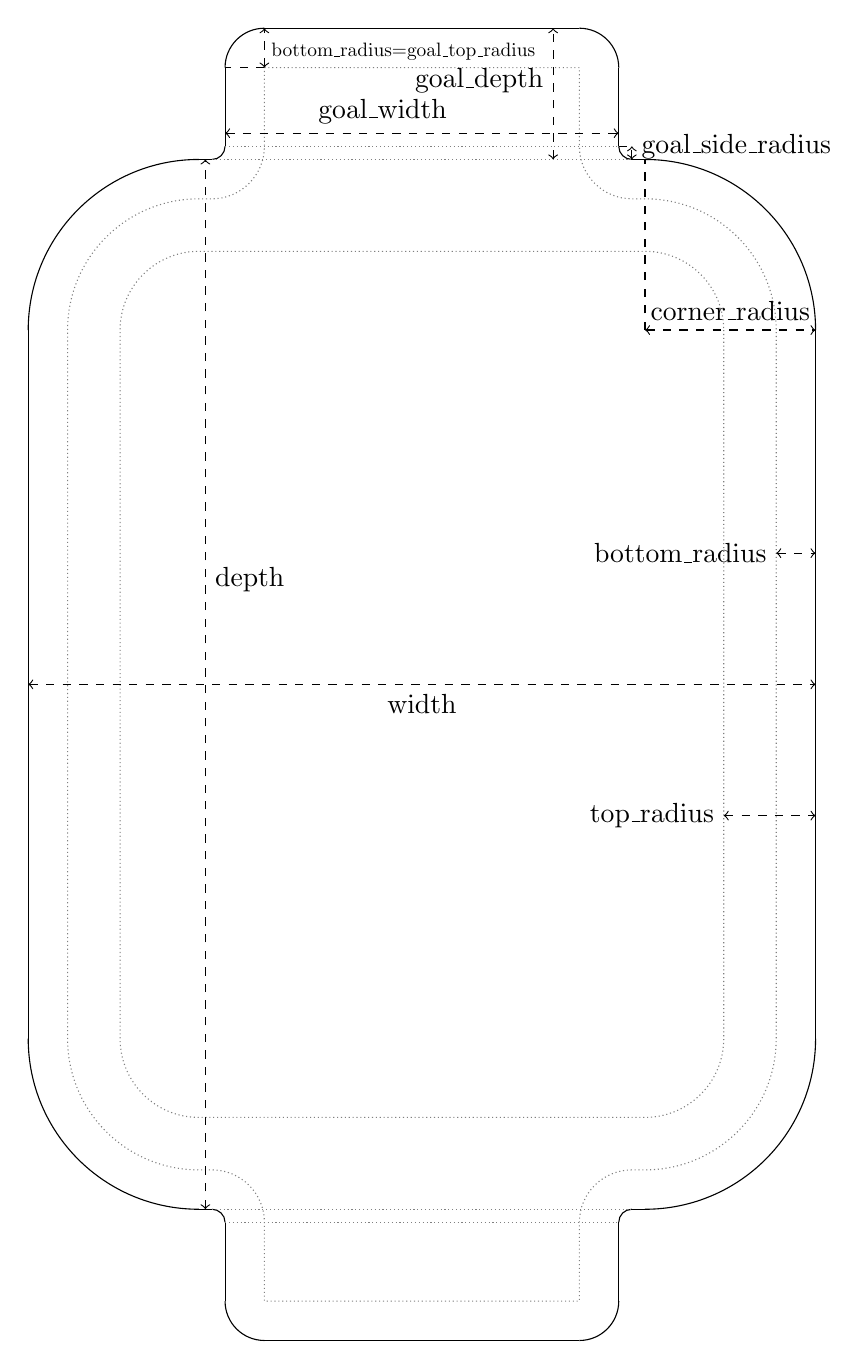
\begin{tikzpicture}[scale=1/6]
      \draw (30,40-13) arc(0:90:13);
      \draw (-30+13,40) arc(90:180:13);
      \draw (-30,-40+13) arc(180:270:13);
      \draw (30-13,-40) arc(270:360:13);
      \draw (30,40-13) -- (30,-40+13);
      \draw (-30,40-13) -- (-30,-40+13);

      \draw (30-13,40) -- (15+1,40);
      \draw (15+1,40) arc(270:180:1);
      \draw (15,41) -- (15,50-3);
      \draw (15,50-3) arc(0:90:3);
      \draw (15-3,50) -- (-15+3,50);
      \draw (-15+3,50) arc(90:180:3);
      \draw (-15,50-3) -- (-15,40+1);
      \draw (-15,40+1) arc(0:-90:1);
      \draw (-16,40) -- (-30+13,40);

      \draw (30-13,-40) -- (15+1,-40);
      \draw (15+1,-40) arc(90:180:1);
      \draw (15,-41) -- (15,-50+3);
      \draw (15,-50+3) arc(0:-90:3);
      \draw (15-3,-50) -- (-15+3,-50);
      \draw (-15+3,-50) arc(270:180:3);
      \draw (-15,-50+3) -- (-15,-40-1);
      \draw (-15,-40-1) arc(0:90:1);
      \draw (-16,-40) -- (-30+13,-40);

      \draw[gray,densely dotted,thin] (-15+3,50-3) -- (15-3,50-3)
            -- (15-3,40+1)
            arc(180:270:3+1)
            -- (30-13,40-3)
            arc(90:0:13-3)
            -- (30-3,-40+13)
            arc(0:-90:13-3)
            -- (15+1,-40+3)
            arc(90:180:3+1)
            -- (15-3,-50+3)
            -- (-15+3,-50+3)
            -- (-15+3,-40-1)
            arc(0:90:3+1)
            -- (-30+13,-40+3)
            arc(270:180:13-3)
            -- (-30+3,40-13)
            arc(180:90:13-3)
            -- (-15-1,40-3)
            arc(-90:0:3+1)
            -- (-15+3,50-3);

      \draw[gray,densely dotted,thin] (30-7,40-13)
            -- (30-7,-40+13)
            arc(0:-90:13-7)
            -- (-30+13,-40+7)
            arc(-90:-180:13-7)
            -- (-30+7,40-13)
            arc(180:90:13-7)
            -- (30-13,40-7)
            arc(90:0:13-7);
      \draw[gray,densely dotted,thin] (-15,40+1) -- (15,40+1);
      \draw[gray,densely dotted,thin] (-15,-40-1) -- (15,-40-1);
      \draw[gray,densely dotted,thin] (-15-1,-40) -- (15+1,-40);

      \draw[<->,dashed] (30-3,10) -- (30,10)
            node[pos=0,left]{bottom\_radius};
      \draw[<->,dashed] (30-7,-10) -- (30,-10)
            node[pos=0,left]{top\_radius};
      \draw[<->,dashed] (30-13,40-13) -- (30,40-13)
            node[pos=0.5,above]{corner\_radius};
      \draw[dashed,thin] (30-13,40-13) -- (30-13,40);
      \draw[<->,dashed] (-30,0) -- (30,0)
            node[pos=0.5,below]{width};
      \draw[<->,dashed] (-16.5,-40) -- (-16.5,40)
            node[pos=0.6,right]{depth};
      \draw[<->,dashed] (15+1,40) -- (15+1,40+1)
            node[pos=1,right]{goal\_side\_radius};
      \draw[dashed,thin] (15,40+1) -- (15+1,40+1);
      \draw[<->,dashed] (-15,42) -- (15,42)
            node[pos=0.4,above]{goal\_width};
      \draw[<->,dashed] (10,40) -- (10,50)
            node[pos=0.6,left]{goal\_depth};
      \draw[gray,densely dotted,thin] (-15-1,40) -- (15+1,40);
      \draw[<->,dashed] (-15+3,50-3) -- (-15+3,50)
            node[pos=0.4,right,scale=0.7]{bottom\_radius=goal\_top\_radius};
      \draw[dashed,thin] (-15+3,50-3) -- (-15,50-3);
\end{tikzpicture}
\caption{Top-down view}
\end{figure}

\begin{figure}[H]
\centering
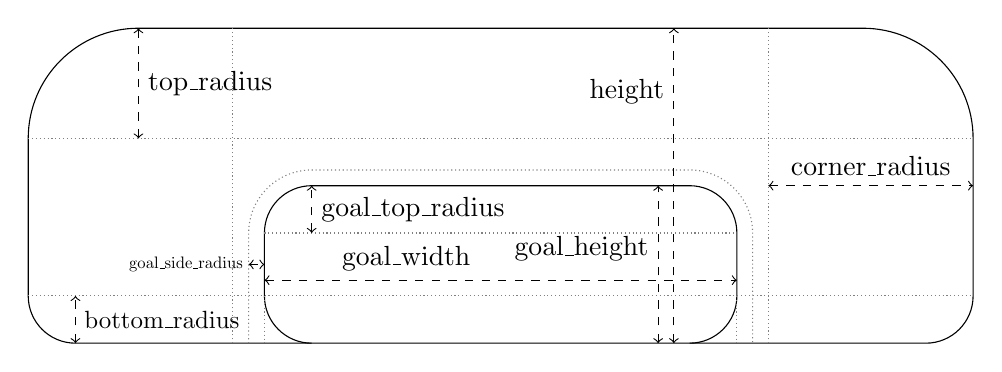
\begin{tikzpicture}[scale=1/5]
      \draw
            (-30,3)
            -- (-30,20-7)
            arc(180:90:7)
            -- (30-7,20)
            arc(90:0:7)
            -- (30,3)
            arc(0:-90:3)
            -- (-30+3,0)
            arc(-90:-180:3);
      
      \draw
            (-15+3,0)
            arc(-90:-180:3)
            -- (-15,10-3)
            arc(180:90:3)
            -- (15-3,10)
            arc(90:0:3)
            -- (15,3)
            arc(0:-90:3);

      \draw[gray,densely dotted,thin]
            (-30,20-7)--(30,20-7);
      \draw[gray,densely dotted,thin]
            (-30,3) -- (30,3);
      \draw[gray,densely dotted,thin]
            (-15,10-3) -- (15,10-3);
      \draw[gray,densely dotted,thin]
            (-15,3) -- (-15,0);
      \draw[gray,densely dotted,thin]
            (15,3) -- (15,0);
      \draw[gray,densely dotted,thin]
            (-15-1,0)
            -- (-15-1,10-3)
            arc(180:90:3+1)
            -- (15-3,10+1)
            arc(90:0:3+1)
            -- (15+1,0);
      \draw[gray,densely dotted,thin] (-30+13,0) -- (-30+13,20);
      \draw[gray,densely dotted,thin] (30-13,0) -- (30-13,20);

      \draw[<->,dashed] (30-13,10) -- (30,10)
            node[pos=0.5,above]{corner\_radius};
      \draw[<->,dashed] (-30+7,20-7) -- (-30+7,20)
            node[pos=0.5,right]{top\_radius};
      \draw[<->,dashed] (-30+3,0) -- (-30+3,3)
            node[pos=0.5,right,scale=0.9]{bottom\_radius};
      \draw[<->,dashed] (-15-1,5) -- (-15,5)
            node[pos=0.0,left,scale=0.6]{goal\_side\_radius};
      \draw[<->,dashed] (-15,4) -- (15,4)
            node[pos=0.3,above]{goal\_width};
      \draw[<->,dashed] (10,0) -- (10,10)
            node[pos=0.6,left]{goal\_height};
      \draw[<->,dashed] (-15+3,10-3) -- (-15+3,10)
            node[pos=0.5,right]{goal\_top\_radius};
      \draw[<->,dashed] (11,0) -- (11,20)
            node[pos=0.8,left]{height};
\end{tikzpicture}
\caption{View on the net}
\end{figure}

\section{Ball and robots}

Ball is a sphere with radius \const{BALL\_RADIUS} and mass \const{BALL\_MASS}.
Coefficient of restitution\footnote{
      The coefficient of restitution is the ratio of the final to
      initial relative velocity between two objects after they collide.
} when the ball collides with the arena is \const{BALL\_ARENA\_E},
so ball loses some speed upon collision.

In the beginning the ball is located in the center of the arena on a random height from the segment
$[\const{BALL\_RADIUS} .. 4\times\const{BALL\_RADIUS}]$.

The ball is considered scored if it completely crosses the net line:
\begin{equation}
      abs(ball.z)>arena.depth/2+ball.radius
\end{equation}
After a scored goal simulation will be reset after \const{RESET\_TICKS} ticks.

Robots are also shperes (with mass \const{ROBOT\_MASS}), but there radius may vary from
\const{ROBOT\_MIN\_RADIUS} to \const{ROBOT\_MAX\_RADIUS},
and is changed while jumping.
The greater jump speed is, the greater the radius.
Exact formula:
\begin{equation}
	\begin{split}
		&radius=\const{ROBOT\_MIN\_RADIUS}+\\
		&(\const{ROBOT\_MAX\_RADIUS}-\const{ROBOT\_MIN\_RADIUS})\times\frac{jump\_speed}{\const{ROBOT\_MAX\_JUMP\_SPEED}}
	\end{split}
\end{equation}

Small increase of the radius while jumping gives robots opportunity to jump off the walls.

Also, while jumping, the simulator thinks, that robot's radius is changing at a constant speed equal to the set jump speed
(even although the radius is actually calculated using the above formula).
This is how jumping is performed.
This way, besides jumping itself, jump speed also has an effect on the strength of hitting the ball.

Coefficient of restitution when robot collides with arena is $0$,
so this kind of collision is absolutely inelastic.
When robot collides with the ball, or with other robots,
coefficient of restitution is equiprobably selected from \const{MIN\_HIT\_E} to \const{MAX\_HIT\_E}.

\section{Nitro}

Beginning with round 2, robots will be allowed to use nitro.
Nitro gives robot acceleration in any direction.
Maximal robot's nitro amount is \const{MAX\_NITRO\_AMOUNT}, one point of nitro changes robot's speed by \const{NITRO\_POINT\_VELOCITY\_CHANGE}.
Using nitro acceleration can't be greater than \const{ROBOT\_NITRO\_ACCELERATION}.

Nitro can be refilled by picking up nitro packs.
Nitro packs are spheres with radius \const{NITRO\_PACK\_RADIUS}, and are considered picked up
if distance betweeb robot's center and nitro pack's center is less than sum of their radii.
Each nitro pack restores nitro back to full (to $100$).
After picked up, the pack will be respawned in the same place after \const{NITRO\_RESPAWN\_TICKS} ticks.
There are $4$ nitro packs total, in points $(\pm\ x, 1, \pm z)$.

In the beginning of the game and after each goal every robot's nitro is equal to \const{START\_NITRO\_AMOUNT}.

In first round nitro is always $0$, and there are no nitro packs.

\section{Control}

Controlling robot means setting target velocity vector, jump speed, and a flag whether nitro should be used.

Without nitro, if robot touches arena,
his velocity will be changing towards target velocity, projected to the touch plane.
Acceleration can not be greater than \const{ROBOT\_ACCELERATION}.
Also, the more vertical the surface, the less acceleration is.
(also, if robot touches arena with its upper half, acceleration is zero).
Thus, when touching the floor, acceleration is maximal, but touching walls or ceiling, it is zero.

When using nitro, velocity also changes towards target velocity, but touching the arena has no effect.

Jump speed can be set from $0$ (don't jump) to \const{ROBOT\_MAX\_JUMP\_SPEED} (jump with max speed).
While jumping, robot's radius is increased slightly, giving him the ability to jump off walls.
Also, while jumping, simulator considers radius to be changing with speed equal to jump speed.
So, jumping is performed because when colliding with the floor, relative velocity in the collition point is equal to jump speed.
This also means than you can control strength of hitting the ball.